\documentclass[11pt]{article}
\usepackage[margin=1in]{geometry}
\usepackage{amsmath,amssymb}
\usepackage{longtable,booktabs,array}
\usepackage{graphicx}
\graphicspath{{plans/active/figures/}{figures/}}
\usepackage{algorithm}
\usepackage{algpseudocode}
\algrenewcommand\algorithmicrequire{\textbf{Input:}}
\algrenewcommand\algorithmicensure{\textbf{Output:}}
\usepackage[hidelinks]{hyperref}
\title{Initial Distributions for a Multi-Agent Housing and Insurance Market:\\A Preliminary Modeling Report}
\author{Preliminary discussion draft}
\date{October 27, 2026}

\begin{document}
\maketitle

\begin{abstract}
We are developing a toy housing and insurance market in which people and competing insurers act as reinforcement-learning agents. Work so far has focused on the environment these agents will face: unequal incomes and property holdings, spatial variation in home values, rental relationships, and disaster risk. We propose initial distributions and simplifying assumptions that make these conditions controllable across experiments. This report presents that modeling work as a basis for studying housing decisions, coverage choices, and insurer pricing. Agent learning and market outcomes remain to be investigated.
\end{abstract}

\section{Goal and work so far}
The goal is a multi-agent market in which people make housing and insurance decisions while insurers compete to sell coverage. A person may rent, own their residence, or hold rental properties. These roles follow from their holdings and can change through market interactions.

Our work so far defines the starting conditions and risk process for this market. We have chosen distributions for income, ownership, and home values; connected people to residences and landlords; and outlined an opening insurance round followed by disaster exposure. These choices establish the environment for subsequent RL experiments, rather than outcomes those agents must produce.

The toy model uses a fixed housing grid, one initial residence per person, and fixed external income without a labor market. Higher-income people tend to occupy more expensive homes and receive larger initial portfolios. Disasters affect a fixed area and destroy the homes within it. These assumptions limit complexity while preserving unequal resources, competing insurance offers, and shared geographic risk.

\begin{figure}[htbp]
\centering
\setlength{\unitlength}{1pt}
\begin{picture}(430,230)
\put(0,202){\makebox(430,18){\textbf{Housing market: ownership and residence}}}
\put(5,148){\framebox(115,34){\shortstack{Person 1\\Owner-occupier}}}
\put(157,148){\framebox(115,34){\shortstack{Person 2\\Landlord}}}
\put(310,148){\framebox(115,34){\shortstack{Person 3\\Renter}}}
\put(5,40){\framebox(115,34){\shortstack{Home A\\Residence of person 1}}}
\put(255,40){\framebox(170,34){\shortstack{Home B\\Residence of person 3}}}
\put(62,148){\vector(0,-1){74}}
\put(65,99){\makebox(90,20)[l]{\scriptsize Owns and occupies}}
\put(214,148){\line(0,-1){48}}
\put(214,100){\line(1,0){77}}
\put(291,100){\vector(0,-1){26}}
\put(222,104){\makebox(53,14){\scriptsize Owns}}
\put(367,148){\vector(0,-1){74}}
\put(371,101){\makebox(55,16)[l]{\scriptsize Occupies}}
\put(310,165){\vector(-1,0){38}}
\put(269,183){\makebox(45,14){\scriptsize Rent}}
\put(0,0){\makebox(430,24){\scriptsize Each home has a grid location and value; ownership and residence are separate.}}
\end{picture}
\caption{Housing relationships: person 1 owns their residence; person 3 rents from person 2. Roles can overlap or change.}
\label{fig:housing-market}
\end{figure}

\section{Mathematical representation and notation}
We represent homes on an $m\times n$ grid, with $H=mn$ homes, $N$ people, and $F$ insurers. Each cell identifies one home and its location. The baseline uses $N=H$ and houses everyone, allowing us to vary inequality while holding housing availability fixed.

The following notation records the resources and relationships agents will encounter. Matrices index homes by location; vectors index people.

\subsection{Definitions and glossary}
Dimensions and indices satisfy
\begin{equation}
\begin{gathered}
 m,n,N,F\in\mathbb{Z}_{>0},\qquad H=mn,\\
 i\in\{1,\ldots,N\},\qquad t\in\mathbb{Z}_{\geq0},\\
 (a,b),(u,v)\in\{1,\ldots,m\}\times\{1,\ldots,n\}.
\end{gathered}
\end{equation}
The housing matrices and personal financial vectors belong to
\begin{equation}
\begin{aligned}
 P &\in \mathbb{R}_{\geq0}^{m\times n},
 & O &\in \{1,\ldots,N\}^{m\times n},\\
 R &\in \{0,\ldots,N\}^{m\times n},
 & D &\in \{0,1\}^{m\times n},\\
 \mathbf{y},\mathbf{c} &\in \mathbb{R}_{\geq0}^{N}.
\end{aligned}
\end{equation}
Indices $(a,b)$ identify homes; $i$ identifies people. Quantities are current unless stated otherwise.

\renewcommand{\arraystretch}{1.12}
\begin{longtable}{@{}p{0.24\textwidth}p{0.69\textwidth}@{}}
\toprule
\textbf{Symbol} & \textbf{Meaning} \\
\midrule
\endfirsthead
\toprule
\textbf{Symbol} & \textbf{Meaning (continued)} \\
\midrule
\endhead
\bottomrule
\endfoot
$P$ & Home values. \\
$O$ & Homeowners, represented by person indices. \\
$R$ & Residents, represented by person indices; zero denotes vacancy. \\
$D$ & Destruction indicators; one denotes a destroyed, uninhabitable home. \\
$\mathbf{y}$ & Fixed annual external incomes. \\
$\mathbf{c}$ & Cash balances. \\
\end{longtable}

Initially, $P\in\mathbb{R}_{>0}^{m\times n}$, $D=0$, and each person appears once in $R$. Ownership indices may repeat. A tenancy occurs where $R_{ab}>0$ and $R_{ab}\ne O_{ab}$. After displacement, a person may have no residence.

The ownership indicator $\mathbf{1}_{\{O_{ab}=i\}}$ identifies homes belonging to person $i$. Their home count and property wealth are
\begin{align}
 \text{home count of person }i &= \sum_{a=1}^{m}\sum_{b=1}^{n}\mathbf{1}_{\{O_{ab}=i\}},\\
 \text{property wealth of person }i &= \sum_{a=1}^{m}\sum_{b=1}^{n}P_{ab}\mathbf{1}_{\{O_{ab}=i\}}.
\end{align}

\begin{figure}[htbp]
\centering
\[
\underbrace{\begin{bmatrix}200&300\\400&500\end{bmatrix}}_{P\text{ (thousands)}}
\qquad
\underbrace{\begin{bmatrix}3&4\\3&4\end{bmatrix}}_{O\text{ (owners)}}
\qquad
\underbrace{\begin{bmatrix}1&2\\3&4\end{bmatrix}}_{R\text{ (residents)}}
\]
\caption{Illustrative allocation: people 1 and 2 rent from 3 and 4. Each owner holds two homes, worth 600 and 800 thousand respectively.}
\label{fig:matrices}
\end{figure}

Contracts link people, insurers, homes, and coverage terms. Their specification, along with rents and insurer capital, remains open.

\subsection{Distribution functions and parameters}
\begin{equation}
\begin{gathered}
 p_0,\mu,\Delta t\in\mathbb{R}_{>0},\qquad
 \sigma,\ell,\tau,\lambda_t\in\mathbb{R}_{\geq0},\qquad S\in\mathbb{Z}_{\geq0},\\
 L_y,L_h:[0,1]\longrightarrow[0,1].
\end{gathered}
\end{equation}
\begin{longtable}{@{}p{0.24\textwidth}p{0.69\textwidth}@{}}
\toprule
\textbf{Symbol} & \textbf{Definition} \\
\midrule
\endfirsthead
\toprule
\textbf{Symbol} & \textbf{Definition (continued)} \\
\midrule
\endhead
\bottomrule
\endfoot
$L_y,L_h$ & Lorenz functions for income and home counts, evaluated along the same person ordering. \\
$\mu,\Delta t$ & Mean annual external income and period length in years. \\
$p_0,\sigma,\ell$ & Reference home price, log-price variation, and spatial smoothing scale. \\
$\tau$ & Noise strength for income-dependent residence placement. \\
$\lambda_t$ & Expected number of disasters in period $t$. \\
$S$ & Global seed, from which labeled component random streams are derived. \\
\end{longtable}

People are indexed by nondecreasing income, with seeded tie-breaking. Auxiliary quantities are defined below.

\section{Assigning initial home values}
We introduce spatial price variation so agents face properties with different values and geographic concentrations of potential loss. A seeded, smoothed Gaussian field generates these initial neighborhoods independently of the population allocation:
\begin{align}
 E_{ab}&\overset{\mathrm{iid}}{\sim}\mathcal{N}(0,1),\\[4pt]
 P&=p_0\exp\left(\sigma\,\mathcal{S}_{\ell}(E)\right).
\end{align}
with $E\in\mathbb{R}^{m\times n}$, an entrywise exponential, and smoothing operator
\begin{align}
 w_{ab,uv}&=\exp\left(-\dfrac{(a-u)^2+(b-v)^2}{2\ell^2}\right),\\[8pt]
 [\mathcal{S}_{\ell}(E)]_{ab}
 &=\dfrac{\displaystyle\sum_{u=1}^{m}\sum_{v=1}^{n}w_{ab,uv}E_{uv}}
 {\displaystyle\sqrt{\sum_{u=1}^{m}\sum_{v=1}^{n}w_{ab,uv}^{2}}}.
\end{align}
For $\ell\in\mathbb{R}_{>0}$, $\ell$ controls neighborhood size; $p_0$ is the marginal median price and $\sigma$ controls spread. Normalization gives unit marginal field variance. Boundaries do not wrap; $\mathcal{S}_0(E)=E$. Initial prices are positive and unbounded above. Market and insurance valuation rules remain separate.

\begin{figure}[htbp]
\centering
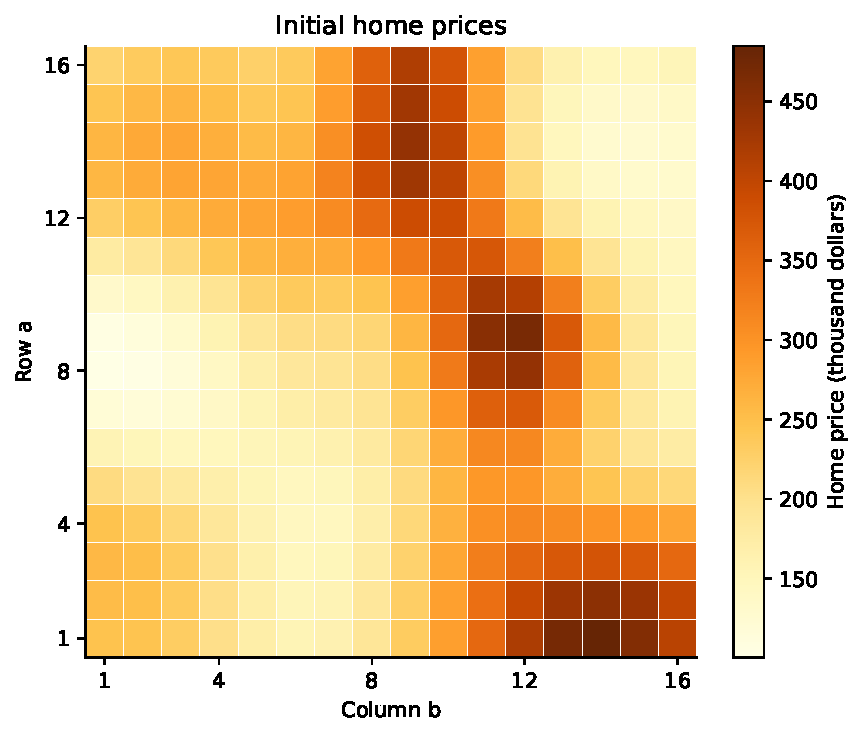
\includegraphics[width=\textwidth]{initial-prices.pdf}
\caption{Illustrative prices: $m=n=16$, $S=42$, $p_0=250{,}000$, $\sigma=0.4$, $\ell=2$. Locations are discrete cells; prices are continuous. The right panel is the analytical marginal density at a fixed cell across seeds, not an empirical density of this spatially correlated map.}
\label{fig:price-distribution}
\end{figure}

\begin{algorithm}[H]
\caption{Generate initial home values}
\label{alg:prices}
\begin{algorithmic}[1]
\Require $m,n,p_0,\sigma,\ell$; price stream derived from seed $S$
\Ensure Price matrix $P$ and destruction matrix $D=0$
\State Draw independent $E_{ab}\sim\mathcal{N}(0,1)$ at every grid cell
\For{each cell $(a,b)$}
    \If{$\ell=0$}
        \State $P_{ab}\gets p_0\exp(\sigma E_{ab})$
    \Else
        \State $w_{ab,uv}\gets\exp\left(-\dfrac{(a-u)^2+(b-v)^2}{2\ell^2}\right)$ for all cells $(u,v)$
        \State $P_{ab}\gets p_0\exp\left(\sigma\dfrac{\sum_{u=1}^m\sum_{v=1}^n w_{ab,uv}E_{uv}}{\sqrt{\sum_{u=1}^m\sum_{v=1}^n w_{ab,uv}^{2}}}\right)$
    \EndIf
    \State $D_{ab}\gets0$
\EndFor
\State \Return $P,D$
\end{algorithmic}
\end{algorithm}

\section{Assigning income and ownership shares}
Unequal income and ownership give agents different starting resources. Two Lorenz curves share the income ranking, linking higher earnings to larger intended portfolios while allowing different concentration levels. Their totals are $N\mu$ dollars per year and $H$ homes.

For either curve, define shares
\begin{equation}
 [\mathbf{d}(L)]_i
 =L\left(\dfrac{i}{N}\right)
 -L\left(\dfrac{i-1}{N}\right),
 \qquad i\in\{1,\ldots,N\}.
\end{equation}
Multiplying these shares by total income or home count gives
\begin{align}
 y_i&=N\mu\left[
 L_y\left(\dfrac{i}{N}\right)-L_y\left(\dfrac{i-1}{N}\right)
 \right],\\[8pt]
 a_i&=H\left[
 L_h\left(\dfrac{i}{N}\right)-L_h\left(\dfrac{i-1}{N}\right)
 \right].
\end{align}
The targets satisfy $\mathbf{a}\in\mathbb{R}_{\geq0}^{N}$. Round them to $\mathbf{h}\in\mathbb{Z}_{\geq0}^{N}$, then correct any difference from $H$:
\begin{enumerate}
\item Round each $a_i$ to the nearest integer, rounding halves upward.
\item If $\sum_i h_i<H$, add one to the count with largest $a_i-h_i$.
\item If $\sum_i h_i>H$, subtract one from a positive count with largest $h_i-a_i$.
\end{enumerate}
Repeat the applicable correction until the total is $H$, recomputing differences and breaking ties by seed. The curve targets counts; property wealth follows from the assigned homes.

Income remains fixed after initialization. Its contribution to cash over one period is
\begin{equation}
 \mathbf{c}\gets\mathbf{c}+\Delta t\,\mathbf{y}.
\end{equation}
Rent and other transactions change cash separately. Starting cash and payment timing remain open.

\begin{figure}[htbp]
\centering
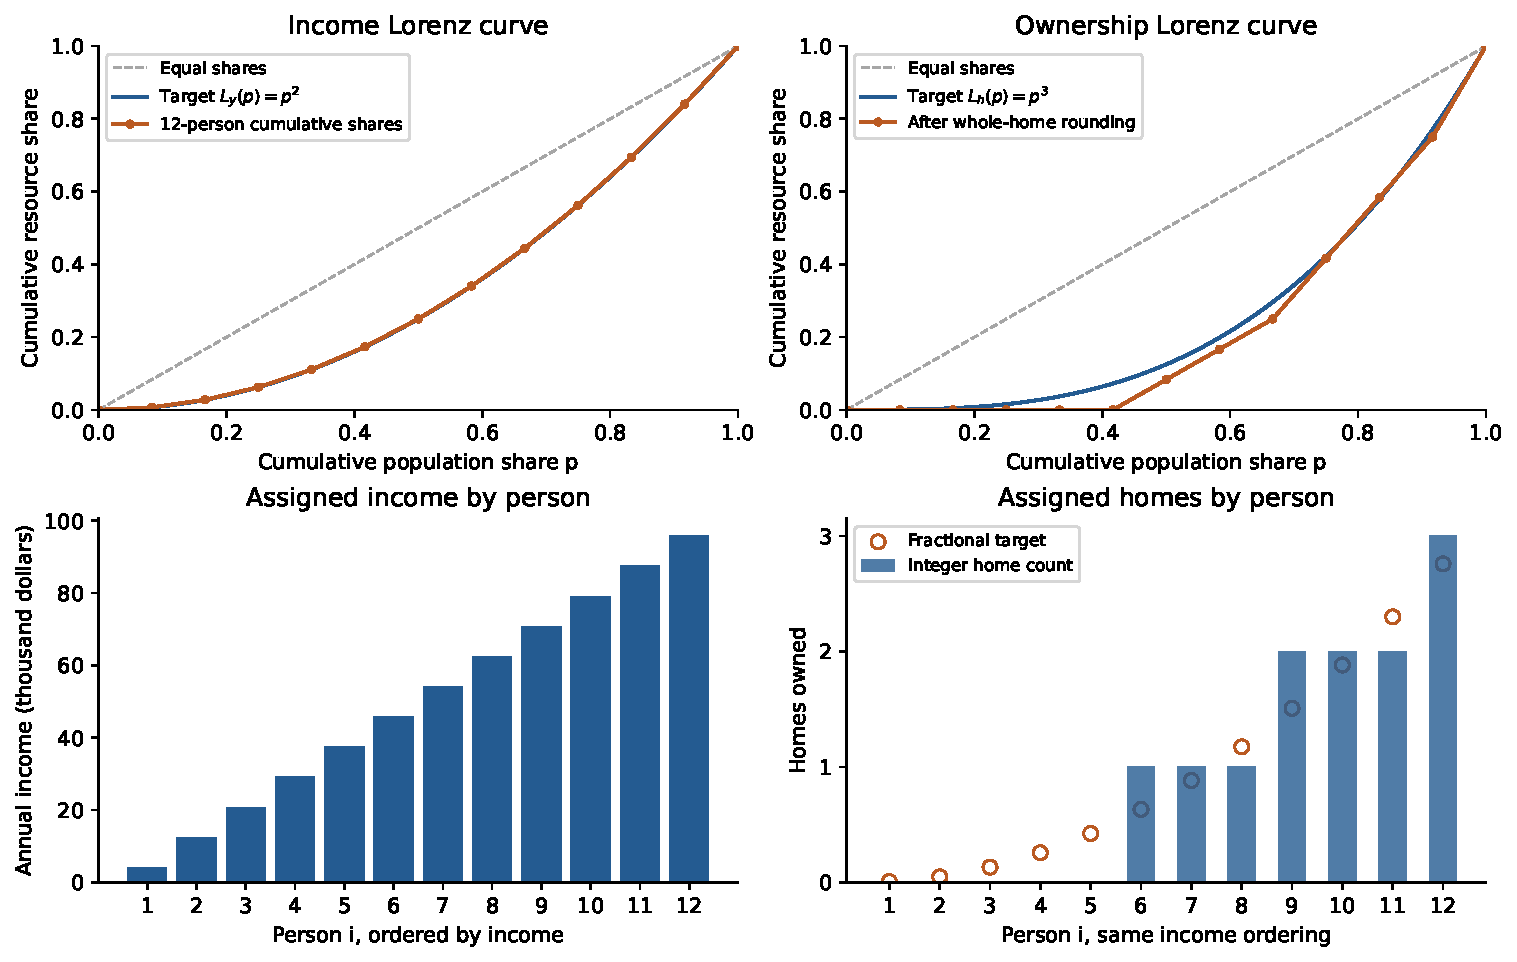
\includegraphics[width=\textwidth]{lorenz-allocations.pdf}
\caption{Illustrative allocations with $N=H=12$, $\mu=50{,}000$, $L_y(p)=p^2$, and $L_h(p)=p^3$; these curves are examples, not selected calibration. Markers show finite-population cumulative shares. Lower panels show assigned annual incomes and whole-home counts, with fractional ownership targets for comparison.}
\label{fig:lorenz-distributions}
\end{figure}

\begin{algorithm}[H]
\caption{Assign fixed incomes and whole-home counts}
\label{alg:incomes}
\begin{algorithmic}[1]
\Require $N,H,\mu,L_y,L_h$; seeded tie-breaking
\Ensure Fixed incomes $\mathbf{y}$ and integer ownership quotas $\mathbf{h}$
\For{$i\in\{1,\ldots,N\}$}
    \State $y_i\gets N\mu\left[L_y\left(\dfrac{i}{N}\right)-L_y\left(\dfrac{i-1}{N}\right)\right]$
    \State $a_i\gets H\left[L_h\left(\dfrac{i}{N}\right)-L_h\left(\dfrac{i-1}{N}\right)\right]$
    \State $h_i\gets\left\lfloor a_i+\dfrac{1}{2}\right\rfloor$
\EndFor
\While{$\sum_{i=1}^N h_i\ne H$}
    \If{$\sum_{i=1}^N h_i<H$}
        \State Select $j\in\arg\max_{i\in\{1,\ldots,N\}}(a_i-h_i)$, breaking ties by seed
        \State $h_j\gets h_j+1$
    \Else
        \State Select $j\in\arg\max_{i:\,h_i>0}(h_i-a_i)$, breaking ties by seed
        \State $h_j\gets h_j-1$
    \EndIf
\EndWhile
\State \Return $\mathbf{y},\mathbf{h}$
\end{algorithmic}
\end{algorithm}

\section{Connecting people to homes}
Residence and ownership determine who pays rent, receives it, or loses housing in a disaster. We assign residences with an income bias while retaining random variation. Scores combine income percentiles $\mathbf{r}\in[0,1]^N$ with Gaussian noise $\mathbf{z}\in\mathbb{R}^N$:
\begin{align}
 z_i&\overset{\mathrm{iid}}{\sim}\mathcal{N}(0,1),\\[4pt]
 q_i&=r_i+\tau z_i,\qquad i\in\{1,\ldots,N\}.
\end{align}
Match people ranked by $\mathbf{q}$ to homes ranked by price. Equal incomes receive equal percentiles; ties are broken by seed. Increasing $\tau$ weakens income-based sorting. An independent baseline uses random assignment.

Second, we assign titles using the quotas from the original income ranking. Each positive-quota owner receives their residence first, then additional homes up to their quota. Nonowners become renters. With $H=N$, residual ownership capacity exactly covers their residences. This assignment does not enforce affordability; initial rents remain open.

Algorithm~\ref{alg:board} uses the generated values, incomes, and quotas. It also requires a rule for choosing among owners with remaining capacity; that choice is still open.

\begin{algorithm}[H]
\caption{Assign residences and ownership}
\label{alg:board}
\begin{algorithmic}[1]
\Require $P,\mathbf{y},\mathbf{h}$; $N=mn$; $\tau$; placement and ownership streams
\Require Residual owner-selection rule
\Ensure Residence matrix $R$ and ownership matrix $O$
\For{$i\in\{1,\ldots,N\}$}
    \State $r_i\gets\dfrac{|\{j:y_j<y_i\}|+\tfrac12|\{j:y_j=y_i\}|}{N}$ \Comment{Midrank percentile}
    \State Draw $z_i\sim\mathcal{N}(0,1)$; set $q_i\gets r_i+\tau z_i$
\EndFor
\State Sort people by $q_i$ and grid cells by $P_{ab}$, resolving ties by seed
\State For each paired person $i$ and cell $(a,b)$, set $R_{ab}\gets i$
\State Set residual capacities $u_i\gets h_i$; initialize $O$ as unassigned
\For{each cell $(a,b)$ with $h_{R_{ab}}>0$}
    \State $O_{ab}\gets R_{ab}$; $u_{R_{ab}}\gets u_{R_{ab}}-1$
\EndFor
\For{each remaining cell $(a,b)$}
    \State Select owner $i$ with $u_i>0$ using the supplied rule and ownership stream
    \State $O_{ab}\gets i$; $u_i\gets u_i-1$
\EndFor
\State Verify $\sum_{a=1}^m\sum_{b=1}^n\mathbf{1}_{\{O_{ab}=i\}}=h_i$ for every person $i$
\State \Return $R,O$
\end{algorithmic}
\end{algorithm}

Starting cash and rent terms are separate inputs to the opening market; their rules remain open. All random streams derive from the global seed. The midrank convention gives equal incomes equal percentiles, including when $N=1$.

\section{Introducing insurance choices}
Insurance connects household decisions to competition among firms. Each of the $F$ insurers can offer homeowners, landlord, and renters coverage; a person's housing relationships determine the applicable products. Firms post offers and people choose contracts before disaster exposure begins. Holding coverage terms fixed while firms adjust premiums is the proposed starting point for studying price competition. Capital, coverage requirements, limits, deductibles, renewals, and settlement rules remain open.

\begin{figure}[htbp]
\centering
\setlength{\unitlength}{1pt}
\begin{picture}(430,275)
\put(0,250){\makebox(430,18){\textbf{Insurance market: people choose among competing firms}}}
\put(5,204){\framebox(125,30){\shortstack{Owner-occupier\\Homeowners coverage}}}
\put(152,204){\framebox(125,30){\shortstack{Landlord\\Landlord coverage}}}
\put(299,204){\framebox(125,30){\shortstack{Renter\\Renters coverage}}}
\put(67,204){\line(0,-1){28}}
\put(214,204){\line(0,-1){28}}
\put(361,204){\line(0,-1){28}}
\put(67,176){\line(1,0){294}}
\put(170,176){\vector(0,-1){54}}
\put(12,146){\makebox(151,18){\scriptsize Premiums}}
\put(340,122){\vector(0,1){54}}
\put(180,125){\makebox(151,40){\shortstack{\scriptsize Offers and covered\\\scriptsize claim payments}}}

\put(5,44){\framebox(419,78){}}
\put(10,98){\makebox(409,18){\small Competing insurer RL agents}}
\put(20,59){\framebox(115,28){Firm A}}
\put(157,59){\framebox(115,28){Firm B}}
\put(294,59){\framebox(115,28){Firm C}}
\put(0,4){\makebox(430,28){\shortstack{\scriptsize Each firm can offer all three products.\\\scriptsize A contract links a person, an insurer, a home, and coverage terms.}}}
\end{picture}
\caption{Housing roles determine applicable coverage. People choose among competing firms; arrows represent market access and contractual payments.}
\label{fig:insurance-market}
\end{figure}

An owner and tenant may insure different losses at the same home with different firms. One disaster can therefore affect several agents and contracts.

\begin{algorithm}[H]
\caption{Establish insurance contracts}
\label{alg:insurance}
\begin{algorithmic}[1]
\Require $P,O,R,D,\mathbf{y},\mathbf{c}$; tenancy records; $F$ firms and initial capital
\Require Product terms, agent policies, eligibility, and payment rules
\Ensure Contract table, updated $\mathbf{c}$, and insurer capital balances
\State Create insurer agents with configured capital
\For{each insurer}
    \State Observe permitted information and post product offers
\EndFor
\For{each person $i$}
    \State Identify applicable products from their entries in $O$ and $R$
    \State Select coverage using the person's policy
\EndFor
\State Validate selections; settle accepted premiums and activate contracts
\State \Return contract table, $\mathbf{c}$, and insurer balances
\end{algorithmic}
\end{algorithm}

\section{Introducing disaster exposure}
Disasters create losses against which agents can seek or sell protection. Poisson counts provide a simple external risk process whose frequency can change while event size stays fixed. Period counts are independent conditional on the rate schedule:
\begin{align}
 K_t&\sim\operatorname{Poisson}(\lambda_t),\\[6pt]
 f(k;\lambda_t)
 &=\Pr(K_t=k)
 =\dfrac{\lambda_t^k e^{-\lambda_t}}{k!},
 \qquad k\in\mathbb{Z}_{\geq0}.
\end{align}
The count satisfies $K_t\in\mathbb{Z}_{\geq0}$; at $\lambda_t=0$, $\Pr(K_t=0)=1$. The rate is expected events per period. Events use a fixed footprint and uniformly sampled eligible centers; shape and boundary treatment remain open.

Let $\mathcal{F}_e\subseteq\{1,\ldots,m\}\times\{1,\ldots,n\}$ contain the cells affected by event $e$. For every $(a,b)\in\mathcal{F}_e$ with $D_{ab}=0$, retain the pre-loss information and set
\begin{align}
 P_{ab}&\gets0,\\
 R_{ab}&\gets0,\\
 D_{ab}&\gets1.
\end{align}
Ownership remains unchanged. The former resident is displaced, and contracts determine covered losses. Checking $D_{ab}=0$ avoids destroying the same unrepaired home twice. Total loss is a simplifying assumption that omits residual land value.

\begin{figure}[htbp]
\centering
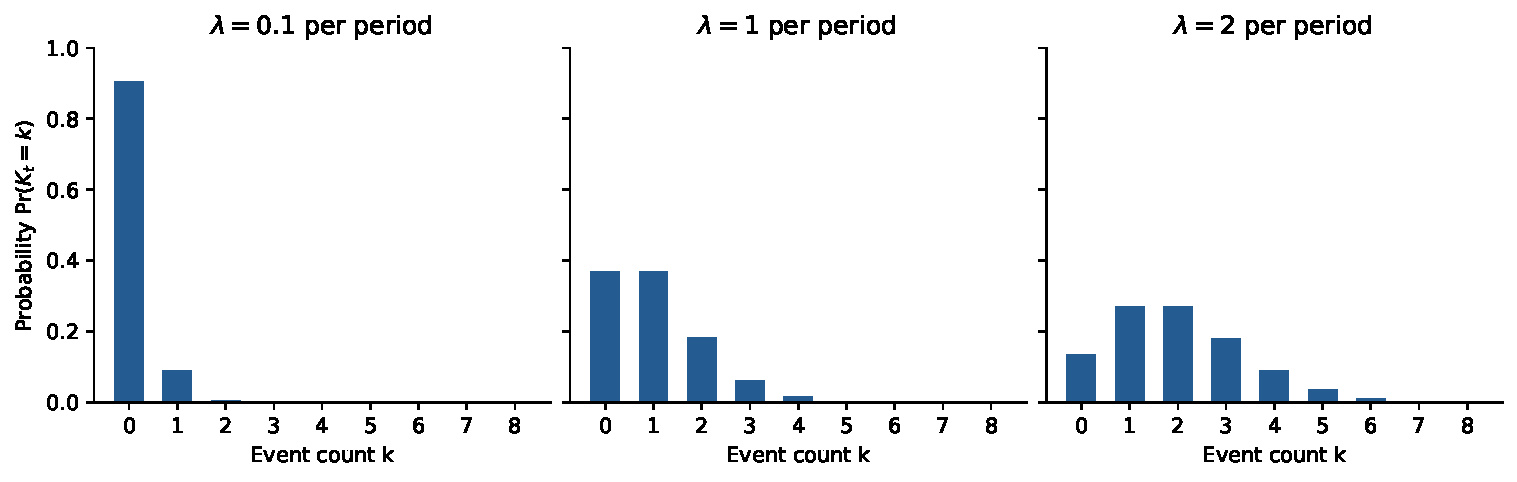
\includegraphics[width=\textwidth]{poisson-counts.pdf}
\caption{Disaster counts per period for illustrative rates, not selected simulation parameters. Displayed probability masses cover $k\in\{0,\ldots,8\}$; the omitted tail is below $0.00024$ in each panel.}
\label{fig:poisson-distribution}
\end{figure}

\begin{algorithm}[H]
\caption{Apply disaster events}
\label{alg:disaster}
\begin{algorithmic}[1]
\Require $P,O,R,D$; contracts; $\lambda_t$; disaster stream
\Require Eligible event centers, fixed footprint, boundary rule, and covered-loss rule
\Ensure Updated $P,R,D$, displacement and loss records; unchanged $O$
\State Draw $K_t\sim\operatorname{Poisson}(\lambda_t)$
\For{$e\in\{1,\ldots,K_t\}$}
    \State Sample an eligible center uniformly; determine affected cells $\mathcal{F}_e$
    \For{each $(a,b)\in\mathcal{F}_e$ with $D_{ab}=0$}
        \State Retain $P_{ab},O_{ab},R_{ab}$ and applicable contracts as pre-loss information
        \If{$R_{ab}>0$}
            \State Record person $R_{ab}$ as displaced
        \EndIf
        \State $P_{ab}\gets0$; $R_{ab}\gets0$; $D_{ab}\gets1$
        \State Record covered losses using the retained information and contract terms
    \EndFor
\EndFor
\State \Return $P,R,D$, displacement records, and loss records
\end{algorithmic}
\end{algorithm}

Within-period ordering, claims timing, replacement housing, and rebuilding remain open.

\section{Next research questions}
The next stage is to define and study agent behavior within this toy market:

\begin{itemize}
\item What observations, actions, and rewards allow people and insurers to learn within this environment?
\item How do income inequality, ownership concentration, and residential sorting change learned behavior and access to coverage?
\item How does disaster frequency affect pricing, displacement, and insurer financial outcomes?
\end{itemize}
Contracts, starting cash, rents, and recovery rules must be settled before training. Experiments will then compare learned interactions across initial conditions and seeds.

\end{document}
